\section{Assembling Long (454) Read}

\begin{note}
The data you will examine in this exercise is again from Staphylococcus aureus
which has a genome of around 3MB. The reads are 454 single end.

The required data can be downloaded from the SRA. Specifically, the run data
(SRR000892, SRR000893) from the SRA Experiment SRX000181.

\center{\url{http://www.ebi.ac.uk/ena/data/view/SRX000181}}
\end{note}

\begin{information}
The following exercise focuses on processing 454 long reads with velvet and how
this differs compared to short reads.
\end{information}

\begin{steps}
First move to the directory you made for this exercise and make a suitable named
directory for the exercise before downloading the read files:
\begin{lstlisting}
cd ~/NGS/velvet/part3
mkdir SRX000181
cd SRX000181
\end{lstlisting}

The downloaded files can be used directly in velvet. To let velvet know that
these FASTQ files are long reads, you pass in the parameter \texttt{-long} by
using the commands:
\begin{lstlisting}
ln -s ~/NGS/Data/SRR000892.fastq.gz
ln -s ~/NGS/Data/SRR000893.fastq.gz
velveth run_25 25 -create_binary -fastq.gz -long *.fastq.gz
time velvetg run_25
\end{lstlisting}
\end{steps}

\begin{questions}
Take a look at the \texttt{stats.txt} file. Which columns are used compared to
short reads and why?
\begin{answer}
long\_cov instead of e.g. short1\_cov
\end{answer}

Which N50 do you get?
\begin{answer}
28 (k-mer N50)
\end{answer}

How long did the \texttt{velvetg} run take?
\begin{answer}
\texttt{real    0m36.333s; user    2m33.238s; sys     0m3.893s}
\end{answer}
\end{questions}

\begin{steps}
The right thing to do is to run \texttt{velvetg} setting the cut-offs. But for long reads
there is an option called \texttt{-long\_cov\_cutoff} to filter them
independently because of the difference in usage in velvet. To investigate with
R, as you did in the previous exercises, start up R and produce the weighted
histogram using the column \texttt{long\_cov} by typing:
\begin{lstlisting}[style=R]
R --no-save
library(plotrix) 
data <- read.table("run_25/stats.txt", header=TRUE) 
weighted.hist(data$long_cov, data$lgth, breaks=0:50)
\end{lstlisting}

\begin{figure}[H]
\centering
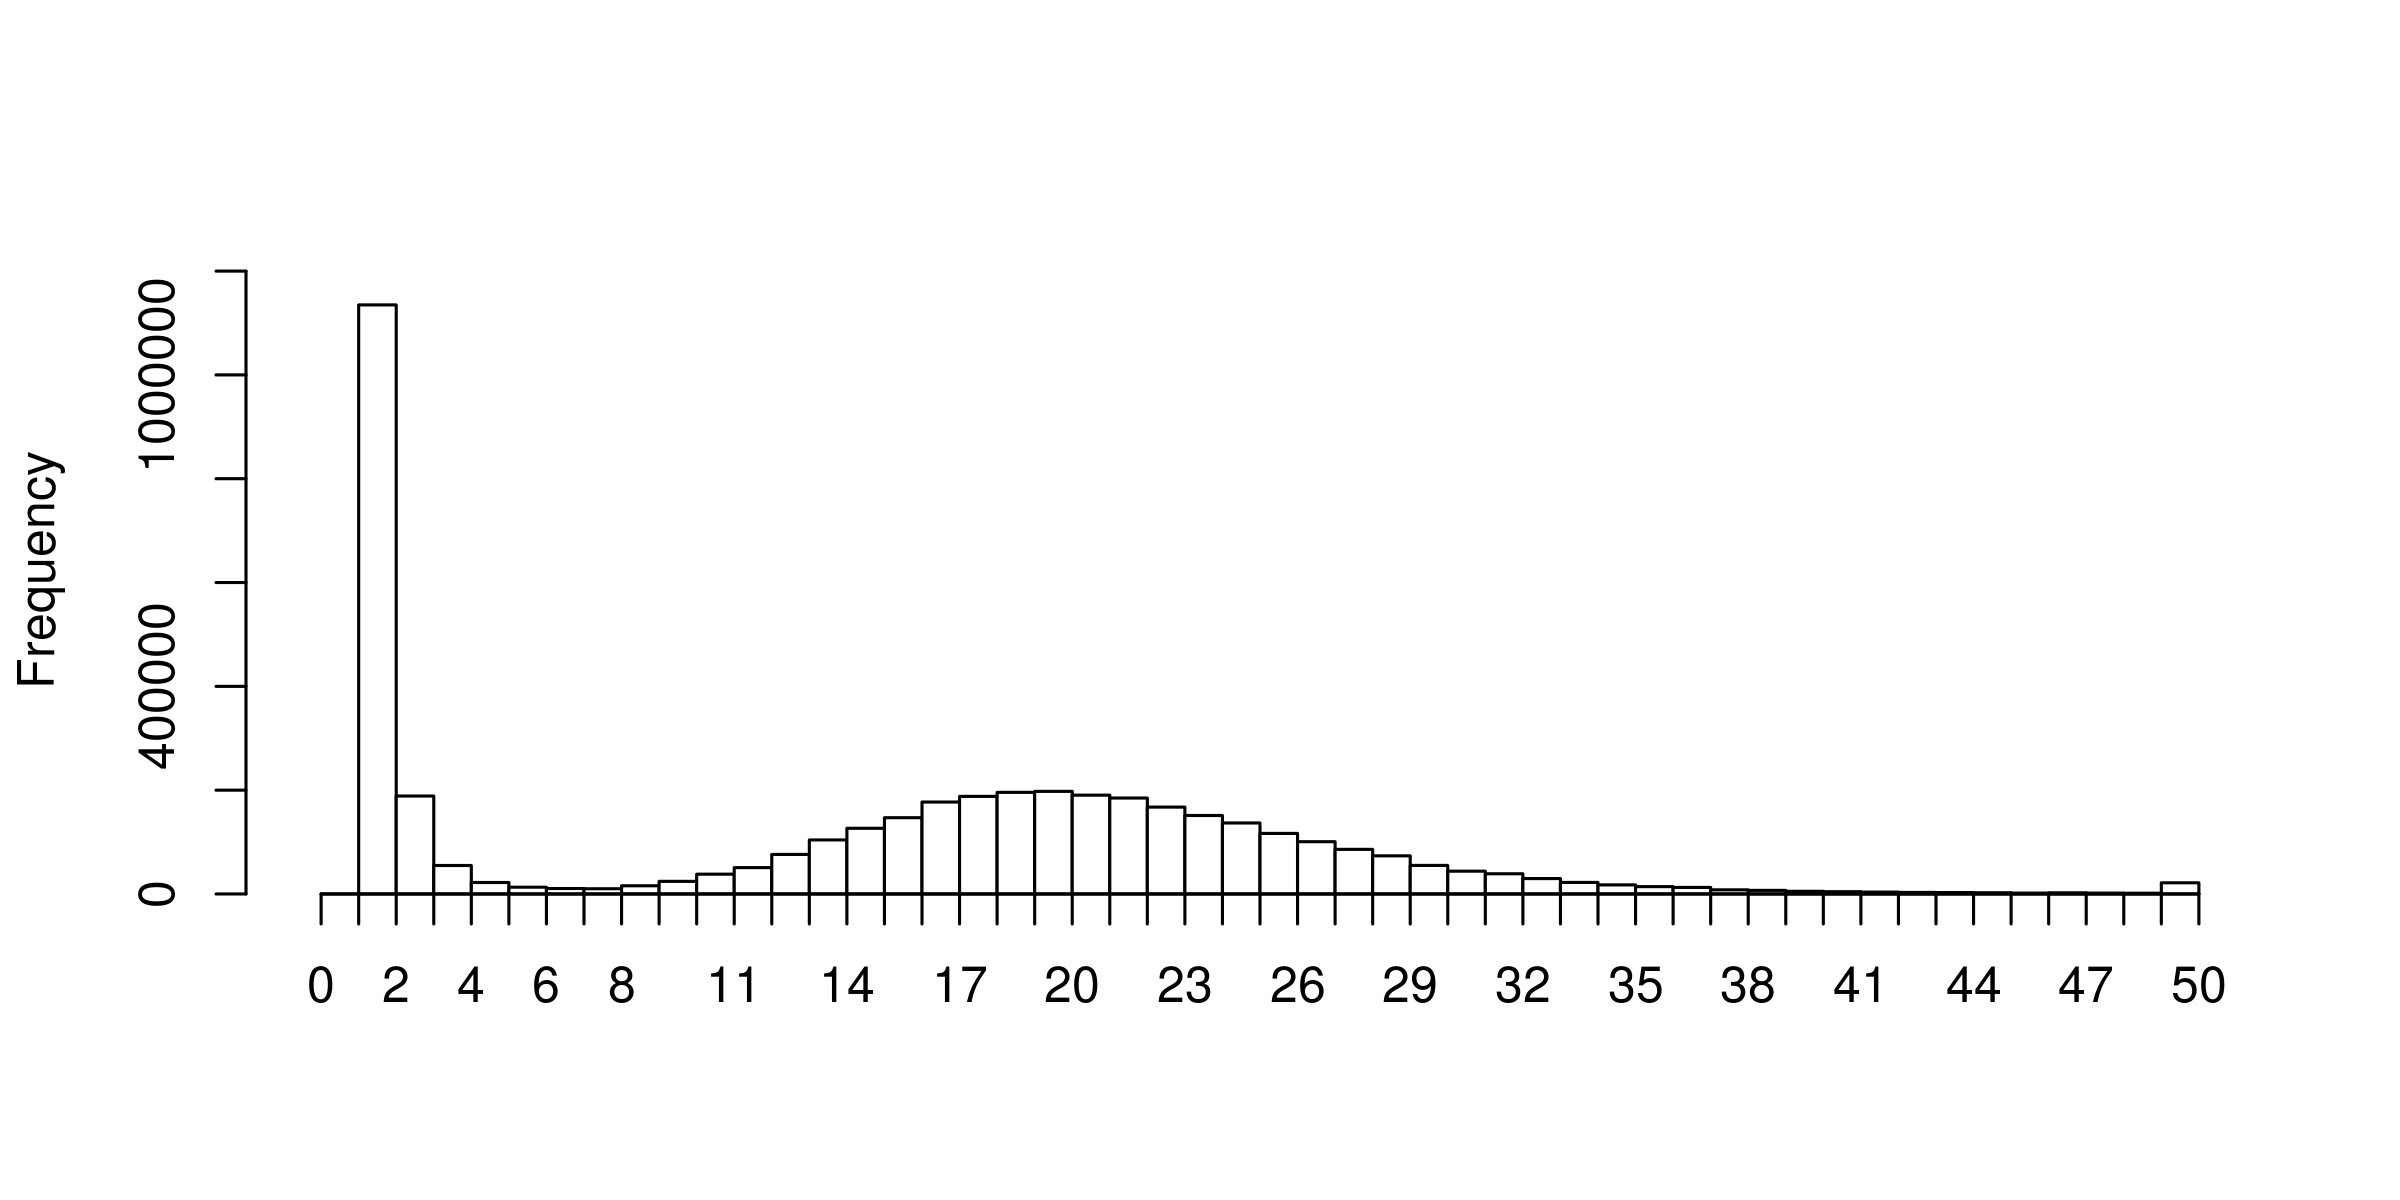
\includegraphics[width=0.8\textwidth]{de_novo/velvet/velvet_Rplot003.png}
\caption{\label{fig:velvetRplot003}}
\end{figure}

For me the histogram suggests to me to choose a coverage cut-off of around 9
with an expected coverage of about 19.

If you disagree, feel free to try different settings, but first leave R before
running \texttt{velvetg}:
\begin{lstlisting}[style=R]
q()
\end{lstlisting}

\begin{lstlisting}
cp run_25/contigs.fa run_25/contigs.fa.0

time velvetg run_25 -long_cov_cutoff 9
cp run_25/contigs.fa run_25/contigs.fa.1

time velvetg run_25 -long_cov_cutoff 9 -exp_cov 19
cp run_25/contigs.fa run_25/contigs.fa.2

gnx -min 100 -nx 25,50,75 run_25/contigs.fa*
\end{lstlisting}

\end{steps}

\begin{questions}
What is the N50 and runtime using:\\
\texttt{-long\_cov\_cutoff 9}
\begin{answer}
\texttt{5,747; real  0m11.457s; user  0m10.855s; sys  0m0.329s}
\end{answer}

\texttt{-long\_cov\_cutoff 9 -exp\_cov 19}
\begin{answer}
\texttt{16,781; real 0m29.830s; user 2m32.530s; sys 0m3.523s}
\end{answer}

other runs?

Which other parameters could improve the assembly quality for long reads?
\begin{answer}
\texttt{-conserveLong}
\end{answer}

What do you think about assembling 454 reads with Velvet?
\begin{answer}
It's working!
\end{answer}
\end{questions}
